\ifpdf
    \graphicspath{{Sections/4_results_figs/Raster/}{Sections/4_results_figs/PDF/}{Sections/4_results_figs/}}
\else
    \graphicspath{{Sections/4_results_figs/Vector/}{Sections/4_results_figs/}}
\fi

\chapter{Results}

\noindent These tables reorganize the CT reconstruction results around implementation,
reconstruction method, and experiment. Super-resolution, deblurring, and denoising-only
results are omitted. Unless stated otherwise, values come from the supplied verification
matrix; Table 7 uses the supplied timing measurements.

\section*{Reporting conventions}
Tables 1--6 show $\mathrm{mean}^{+u}_{-l}$ with asymmetric 95\% bootstrap confidence
intervals (2,000 resamples). Bold marks the best displayed value, including ties. RSR is
relative sinogram residual; PC is predictor--corrector. Paper, Public-compatible, and
LION-physics identify implementations. Test size is
$n=25$, except Table 3 ($n=4$). Table 7 has no intervals.

\clearpage

\begin{landscape}
\begin{table}[p]
\centering
\caption{CT reconstruction (360 Degrees; cond.: noise-conditioned DRUnet).}\label{tab:main-quality}
\small
\setlength{\tabcolsep}{2.4pt}
\resizebox{\linewidth}{!}{%
\begin{tabular}{lllcccccccc}
\toprule[1.1pt]
\multicolumn{1}{c}{\bfseries Implementation} & \multicolumn{2}{c}{\bfseries Reconstruction method} & \multicolumn{4}{c}{\bfseries 20-View 360 Degrees} & \multicolumn{4}{c}{\bfseries 8-View 360 Degrees} \\
\cmidrule(lr){2-3} \cmidrule(lr){4-7} \cmidrule(lr){8-11}
 & \textbf{Sampler} & \textbf{Prior} & \textbf{PSNR} & \textbf{SSIM} & \textbf{MAE} & \textbf{RSR} & \textbf{PSNR} & \textbf{SSIM} & \textbf{MAE} & \textbf{RSR} \\
\midrule
\textbf{Paper} & VE--DPS & Whole-Image & $33.97^{+0.70}_{-0.63}$ & $0.825^{+0.021}_{-0.023}$ & $0.0137^{+0.0010}_{-0.0010}$ & $0.0373^{+0.0026}_{-0.0026}$ & $29.10^{+0.78}_{-0.78}$ & $0.743^{+0.023}_{-0.024}$ & $0.0195^{+0.0015}_{-0.0015}$ & $0.0330^{+0.0038}_{-0.0036}$ \\
 & Langevin & PaDIS & $30.74^{+0.84}_{-0.90}$ & $0.680^{+0.041}_{-0.047}$ & $0.0221^{+0.0026}_{-0.0026}$ & $0.0800^{+0.0132}_{-0.0125}$ & $26.08^{+0.52}_{-0.47}$ & $0.589^{+0.035}_{-0.041}$ & $0.0295^{+0.0021}_{-0.0020}$ & $0.0542^{+0.0066}_{-0.0068}$ \\
 & PC & PaDIS & $25.46^{+0.22}_{-0.22}$ & $0.412^{+0.019}_{-0.019}$ & $0.0371^{+0.0011}_{-0.0011}$ & $0.0732^{+0.0060}_{-0.0069}$ & $22.30^{+0.38}_{-0.39}$ & $0.330^{+0.010}_{-0.010}$ & $0.0502^{+0.0022}_{-0.0020}$ & $0.0469^{+0.0039}_{-0.0045}$ \\
 & VE--DDNM & PaDIS & $29.13^{+1.02}_{-0.94}$ & $0.651^{+0.040}_{-0.046}$ & $0.0250^{+0.0029}_{-0.0028}$ & $0.0059^{+0.0008}_{-0.0008}$ & $22.42^{+0.38}_{-0.39}$ & $0.330^{+0.029}_{-0.031}$ & $0.0505^{+0.0028}_{-0.0027}$ & $0.0320^{+0.0038}_{-0.0034}$ \\
 & VE--DPS & PaDIS & $32.71^{+0.82}_{-0.85}$ & $0.777^{+0.038}_{-0.042}$ & $0.0160^{+0.0020}_{-0.0018}$ & $0.0312^{+0.0079}_{-0.0071}$ & $27.15^{+0.72}_{-0.72}$ & $0.669^{+0.039}_{-0.041}$ & $0.0246^{+0.0026}_{-0.0024}$ & $0.0227^{+0.0050}_{-0.0043}$ \\
\addlinespace[2pt]\midrule
\textbf{Public-compatible} & Langevin & PaDIS & $31.86^{+0.79}_{-0.77}$ & $0.795^{+0.033}_{-0.036}$ & $0.0165^{+0.0018}_{-0.0017}$ & $0.0353^{+0.0025}_{-0.0025}$ & $23.88^{+0.78}_{-0.74}$ & $0.553^{+0.032}_{-0.032}$ & $0.0402^{+0.0038}_{-0.0035}$ & $0.0341^{+0.0025}_{-0.0024}$ \\
 & PC & PaDIS & $28.15^{+0.34}_{-0.34}$ & $0.627^{+0.027}_{-0.028}$ & $0.0264^{+0.0013}_{-0.0013}$ & $0.0705^{+0.0083}_{-0.0076}$ & $23.86^{+0.62}_{-0.57}$ & $0.462^{+0.021}_{-0.018}$ & $0.0423^{+0.0029}_{-0.0029}$ & $0.0335^{+0.0037}_{-0.0039}$ \\
 & VE--DDNM & PaDIS & $30.00^{+1.13}_{-1.09}$ & $0.712^{+0.054}_{-0.057}$ & $0.0215^{+0.0038}_{-0.0032}$ & $0.0048^{+0.0005}_{-0.0005}$ & $25.85^{+0.67}_{-0.64}$ & $0.602^{+0.040}_{-0.044}$ & $0.0300^{+0.0030}_{-0.0029}$ & $0.0061^{+0.0004}_{-0.0004}$ \\
 & VE--DPS & Patch avg. & $35.77^{+0.32}_{-0.39}$ & $0.882^{+0.023}_{-0.021}$ & $0.0102^{+0.0008}_{-0.0005}$ & $0.0266^{+0.0061}_{-0.0059}$ & $29.05^{+1.73}_{-1.43}$ & $0.778^{+0.044}_{-0.048}$ & $0.0179^{+0.0030}_{-0.0029}$ & $0.0171^{+0.0053}_{-0.0041}$ \\
 & VE--DPS & Patch stitch. & $35.04^{+0.34}_{-0.19}$ & $0.889^{+0.011}_{-0.021}$ & $0.0109^{+0.0003}_{-0.0002}$ & $0.0353^{+0.0092}_{-0.0120}$ & $27.79^{+1.15}_{-1.15}$ & $0.741^{+0.028}_{-0.025}$ & $0.0206^{+0.0023}_{-0.0023}$ & $0.0144^{+0.0021}_{-0.0021}$ \\
 & VE--DPS & PaDIS & $32.49^{+1.15}_{-1.15}$ & $0.805^{+0.039}_{-0.045}$ & $0.0156^{+0.0023}_{-0.0021}$ & $0.0187^{+0.0027}_{-0.0024}$ & $25.50^{+0.75}_{-0.78}$ & $0.619^{+0.041}_{-0.042}$ & $0.0307^{+0.0037}_{-0.0034}$ & $0.0135^{+0.0010}_{-0.0010}$ \\
\addlinespace[2pt]\midrule
\textbf{LION-physics} & FBP & -- & $23.35^{+0.77}_{-0.73}$ & $0.439^{+0.020}_{-0.018}$ & $0.0483^{+0.0039}_{-0.0039}$ & $0.1008^{+0.0132}_{-0.0142}$ & $19.09^{+0.89}_{-0.80}$ & $0.305^{+0.019}_{-0.018}$ & $0.0796^{+0.0069}_{-0.0069}$ & $0.2288^{+0.0321}_{-0.0355}$ \\
 & ADMM & TV & $28.62^{+0.52}_{-0.52}$ & $0.738^{+0.018}_{-0.018}$ & $0.0221^{+0.0016}_{-0.0016}$ & $0.0113^{+0.0012}_{-0.0012}$ & $24.38^{+0.74}_{-0.66}$ & $0.582^{+0.024}_{-0.022}$ & $0.0410^{+0.0039}_{-0.0041}$ & $0.0249^{+0.0043}_{-0.0043}$ \\
 & PnP--ADMM & DRUnet (cond) & $26.12^{+1.18}_{-1.23}$ & $0.620^{+0.047}_{-0.049}$ & $0.0314^{+0.0042}_{-0.0040}$ & $0.0093^{+0.0051}_{-0.0042}$ & $17.26^{+1.09}_{-1.20}$ & $0.291^{+0.060}_{-0.060}$ & $0.0889^{+0.0210}_{-0.0187}$ & $0.1236^{+0.0627}_{-0.0509}$ \\
 & PnP--ADMM & DRUnet & $26.12^{+1.14}_{-1.20}$ & $0.620^{+0.047}_{-0.047}$ & $0.0315^{+0.0042}_{-0.0036}$ & $0.0093^{+0.0053}_{-0.0044}$ & $17.93^{+0.88}_{-0.92}$ & $0.320^{+0.053}_{-0.058}$ & $0.0777^{+0.0126}_{-0.0117}$ & $0.0813^{+0.0263}_{-0.0202}$ \\
 & VE--DPS & Whole-Image & $34.25^{+0.69}_{-0.64}$ & $0.865^{+0.022}_{-0.024}$ & $0.0118^{+0.0010}_{-0.0011}$ & $0.0014^{+0.0001}_{-0.0001}$ & $\mathbf{29.58^{+0.69}_{-0.63}}$ & $0.783^{+0.021}_{-0.024}$ & $0.0175^{+0.0012}_{-0.0012}$ & $\mathbf{0.0012^{+0.0001}_{-0.0001}}$ \\
 & Langevin & PaDIS & $31.62^{+0.95}_{-0.97}$ & $0.788^{+0.047}_{-0.050}$ & $0.0167^{+0.0029}_{-0.0024}$ & $0.0015^{+0.0001}_{-0.0001}$ & $26.16^{+0.55}_{-0.54}$ & $0.652^{+0.041}_{-0.043}$ & $0.0272^{+0.0025}_{-0.0024}$ & $0.0014^{+0.0002}_{-0.0002}$ \\
 & Langevin & Whole-Image & $33.26^{+0.64}_{-0.62}$ & $0.851^{+0.020}_{-0.022}$ & $0.0128^{+0.0011}_{-0.0011}$ & $0.0017^{+0.0001}_{-0.0001}$ & -- & -- & -- & -- \\
 & PC & PaDIS & $28.58^{+0.43}_{-0.45}$ & $0.691^{+0.025}_{-0.027}$ & $0.0228^{+0.0013}_{-0.0012}$ & $0.0072^{+0.0005}_{-0.0005}$ & $24.41^{+0.49}_{-0.50}$ & $0.555^{+0.020}_{-0.020}$ & $0.0347^{+0.0021}_{-0.0020}$ & $0.0077^{+0.0005}_{-0.0006}$ \\
 & PC & Whole-Image & $28.91^{+0.32}_{-0.31}$ & $0.585^{+0.014}_{-0.014}$ & $0.0242^{+0.0008}_{-0.0009}$ & $0.0208^{+0.0029}_{-0.0026}$ & -- & -- & -- & -- \\
 & VE--DDNM & PaDIS & $\mathbf{36.49^{+1.01}_{-0.95}}$ & $0.895^{+0.021}_{-0.023}$ & $0.0103^{+0.0012}_{-0.0011}$ & $\mathbf{0.0013^{+0.0002}_{-0.0002}}$ & $27.12^{+0.66}_{-0.64}$ & $0.670^{+0.033}_{-0.035}$ & $0.0265^{+0.0021}_{-0.0021}$ & $0.0112^{+0.0018}_{-0.0017}$ \\
 & VE--DDNM & Whole-Image & $34.19^{+1.13}_{-1.09}$ & $0.835^{+0.034}_{-0.038}$ & $0.0136^{+0.0019}_{-0.0017}$ & $0.0025^{+0.0003}_{-0.0002}$ & -- & -- & -- & -- \\
 & VE--DPS & Patch avg. & $36.10^{+1.40}_{-1.52}$ & $\mathbf{0.914^{+0.029}_{-0.051}}$ & $\mathbf{0.0087^{+0.0024}_{-0.0015}}$ & $0.0014^{+0.0003}_{-0.0003}$ & $29.05^{+1.28}_{-1.19}$ & $\mathbf{0.805^{+0.045}_{-0.068}}$ & $\mathbf{0.0167^{+0.0034}_{-0.0025}}$ & $0.0015^{+0.0003}_{-0.0003}$ \\
 & VE--DPS & Patch stitch. & $34.23^{+1.45}_{-1.10}$ & $0.888^{+0.040}_{-0.039}$ & $0.0107^{+0.0017}_{-0.0017}$ & $0.0018^{+0.0004}_{-0.0004}$ & $27.96^{+0.68}_{-0.68}$ & $0.773^{+0.020}_{-0.018}$ & $0.0191^{+0.0009}_{-0.0014}$ & $0.0020^{+0.0004}_{-0.0004}$ \\
 & VE--DPS & PaDIS & $32.82^{+1.00}_{-1.04}$ & $0.816^{+0.041}_{-0.049}$ & $0.0148^{+0.0025}_{-0.0022}$ & $\mathbf{0.0013^{+0.0001}_{-0.0001}}$ & $27.65^{+0.80}_{-0.80}$ & $0.706^{+0.043}_{-0.049}$ & $0.0229^{+0.0025}_{-0.0024}$ & $\mathbf{0.0012^{+0.0002}_{-0.0002}}$ \\
\bottomrule[1.1pt]
\end{tabular}
}
\end{table}
\end{landscape}
\clearpage

\begin{landscape}
\begin{table}[p]
\centering
\caption{CT reconstruction: additional geometries.}\label{tab:extra-quality}
\small
\setlength{\tabcolsep}{2.4pt}
\resizebox{\linewidth}{!}{%
\begin{tabular}{lllcccccccc}
\toprule[1.1pt]
\multicolumn{1}{c}{\bfseries Implementation} & \multicolumn{2}{c}{\bfseries Reconstruction method} & \multicolumn{4}{c}{\bfseries 60-View 360 Degrees} & \multicolumn{4}{c}{\bfseries 20-View 120 Degrees} \\
\cmidrule(lr){2-3} \cmidrule(lr){4-7} \cmidrule(lr){8-11}
 & \textbf{Sampler} & \textbf{Prior} & \textbf{PSNR} & \textbf{SSIM} & \textbf{MAE} & \textbf{RSR} & \textbf{PSNR} & \textbf{SSIM} & \textbf{MAE} & \textbf{RSR} \\
\midrule
\textbf{Paper} & VE--DDNM & PaDIS & $36.70^{+1.52}_{-1.48}$ & $0.874^{+0.029}_{-0.032}$ & $0.0116^{+0.0019}_{-0.0017}$ & $0.0030^{+0.0003}_{-0.0003}$ & $26.79^{+0.75}_{-0.73}$ & $0.590^{+0.035}_{-0.037}$ & $0.0298^{+0.0027}_{-0.0026}$ & $0.0117^{+0.0018}_{-0.0016}$ \\
\addlinespace[2pt]\midrule
\textbf{Public-compatible} & VE--DDNM & PaDIS & $32.71^{+1.64}_{-1.83}$ & $0.781^{+0.060}_{-0.065}$ & $0.0174^{+0.0041}_{-0.0035}$ & $0.0044^{+0.0006}_{-0.0006}$ & $27.18^{+0.68}_{-0.70}$ & $0.650^{+0.047}_{-0.049}$ & $0.0263^{+0.0031}_{-0.0029}$ & $0.0066^{+0.0007}_{-0.0006}$ \\
 & VE--DPS & PaDIS & $36.38^{+1.00}_{-1.09}$ & $0.876^{+0.025}_{-0.028}$ & $0.0112^{+0.0015}_{-0.0013}$ & $0.0288^{+0.0036}_{-0.0032}$ & $28.19^{+0.67}_{-0.65}$ & $0.750^{+0.033}_{-0.035}$ & $0.0207^{+0.0019}_{-0.0018}$ & $0.0194^{+0.0020}_{-0.0019}$ \\
\addlinespace[2pt]\midrule
\textbf{LION-physics} & FBP & -- & $29.05^{+0.49}_{-0.48}$ & $0.646^{+0.018}_{-0.016}$ & $0.0240^{+0.0015}_{-0.0015}$ & $0.0287^{+0.0036}_{-0.0037}$ & $20.17^{+0.24}_{-0.22}$ & $0.481^{+0.018}_{-0.017}$ & $0.0680^{+0.0019}_{-0.0019}$ & $0.2146^{+0.0094}_{-0.0094}$ \\
 & ADMM & TV & $31.65^{+0.43}_{-0.43}$ & $0.835^{+0.021}_{-0.022}$ & $0.0145^{+0.0009}_{-0.0009}$ & $0.0099^{+0.0010}_{-0.0009}$ & $25.80^{+0.68}_{-0.65}$ & $0.689^{+0.017}_{-0.016}$ & $0.0328^{+0.0026}_{-0.0027}$ & $0.0127^{+0.0014}_{-0.0015}$ \\
 & VE--DPS & Whole-Image & $37.99^{+0.87}_{-0.88}$ & $0.919^{+0.018}_{-0.022}$ & $0.0085^{+0.0012}_{-0.0010}$ & $0.0022^{+0.0001}_{-0.0001}$ & $\mathbf{30.83^{+0.45}_{-0.48}}$ & $\mathbf{0.835^{+0.019}_{-0.021}}$ & $\mathbf{0.0146^{+0.0010}_{-0.0010}}$ & $0.0016^{+0.0002}_{-0.0002}$ \\
 & VE--DDNM & PaDIS & $\mathbf{41.55^{+1.53}_{-1.55}}$ & $\mathbf{0.951^{+0.014}_{-0.016}}$ & $\mathbf{0.0066^{+0.0012}_{-0.0011}}$ & $\mathbf{0.0012^{+0.0001}_{-0.0001}}$ & $29.96^{+0.95}_{-0.89}$ & $0.780^{+0.032}_{-0.032}$ & $0.0187^{+0.0021}_{-0.0020}$ & $0.0053^{+0.0015}_{-0.0013}$ \\
 & VE--DPS & PaDIS & $37.12^{+1.27}_{-1.38}$ & $0.895^{+0.033}_{-0.036}$ & $0.0099^{+0.0019}_{-0.0018}$ & $0.0021^{+0.0001}_{-0.0001}$ & $29.03^{+0.61}_{-0.63}$ & $0.770^{+0.040}_{-0.042}$ & $0.0188^{+0.0022}_{-0.0019}$ & $\mathbf{0.0015^{+0.0001}_{-0.0001}}$ \\
\bottomrule[1.1pt]
\end{tabular}
}
\end{table}
\end{landscape}
\clearpage

\begin{table}[p]
\centering
\caption{$512\times512$ CT reconstruction (60-View 360 Degrees).}\label{tab:ct512}
\small
\normalsize
\setlength{\tabcolsep}{2pt}
\resizebox{\linewidth}{!}{%
\begin{tabular}{lllcccc}
\toprule[1.1pt]
\multicolumn{1}{c}{\bfseries Implementation} & \multicolumn{2}{c}{\bfseries Reconstruction method} & \multicolumn{4}{c}{\bfseries $512\times512$, 60-View 360 Degrees} \\
\cmidrule(lr){2-3} \cmidrule(lr){4-7}
 & \textbf{Sampler} & \textbf{Prior} & \textbf{PSNR} & \textbf{SSIM} & \textbf{MAE} & \textbf{RSR} \\
\midrule
\textbf{Public-compatible} & VE--DPS & PaDIS & $39.24^{+0.12}_{-0.11}$ & $0.922^{+0.007}_{-0.004}$ & $0.0071^{+0.0003}_{-0.0003}$ & $0.0243^{+0.0041}_{-0.0046}$ \\
\addlinespace[2pt]\midrule
\textbf{LION-physics} & FBP & -- & $29.86^{+0.62}_{-0.62}$ & $0.699^{+0.036}_{-0.036}$ & $0.0205^{+0.0016}_{-0.0016}$ & $0.0344^{+0.0096}_{-0.0096}$ \\
 & ADMM & TV & $33.77^{+0.77}_{-0.77}$ & $0.904^{+0.007}_{-0.007}$ & $0.0103^{+0.0004}_{-0.0004}$ & $0.0074^{+0.0017}_{-0.0017}$ \\
 & VE--DPS & PaDIS & $\mathbf{40.08^{+0.71}_{-1.11}}$ & $\mathbf{0.960^{+0.004}_{-0.004}}$ & $\mathbf{0.0056^{+0.0003}_{-0.0003}}$ & $\mathbf{0.0018^{+0.0003}_{-0.0003}}$ \\
\bottomrule[1.1pt]
\end{tabular}
}
\end{table}
\clearpage

\begin{table}[p]
\centering
\caption{VE--DPS patch-size ablation (20-View 360 Degrees; unmarked: PaDIS).}\label{tab:patch-size}
\small
\normalsize
\setlength{\tabcolsep}{2pt}
\resizebox{\linewidth}{!}{%
\begin{tabular}{llcccc}
\toprule[1.1pt]
\multicolumn{1}{c}{\bfseries Implementation} & \multicolumn{1}{c}{\bfseries Patch size} & \multicolumn{4}{c}{\bfseries 20-View 360 Degrees} \\
\cmidrule(lr){3-6}
 &  & \textbf{PSNR} & \textbf{SSIM} & \textbf{MAE} & \textbf{RSR} \\
\midrule
\textbf{Paper} & $P=256$ (Whole-Image) & $33.97^{+0.70}_{-0.63}$ & $0.825^{+0.021}_{-0.023}$ & $0.0137^{+0.0010}_{-0.0010}$ & $0.0373^{+0.0026}_{-0.0026}$ \\
\addlinespace[2pt]\midrule
\textbf{Public-compatible} & $P=8$ & $31.66^{+0.70}_{-0.78}$ & $0.801^{+0.020}_{-0.020}$ & $0.0162^{+0.0015}_{-0.0014}$ & $0.0169^{+0.0024}_{-0.0020}$ \\
 & $P=16$ & $30.66^{+0.66}_{-0.73}$ & $0.746^{+0.028}_{-0.031}$ & $0.0189^{+0.0017}_{-0.0017}$ & $0.0170^{+0.0026}_{-0.0023}$ \\
 & $P=32$ & $28.97^{+0.86}_{-0.88}$ & $0.676^{+0.044}_{-0.046}$ & $0.0239^{+0.0027}_{-0.0028}$ & $0.0202^{+0.0031}_{-0.0030}$ \\
 & $P=56$ & $32.49^{+1.11}_{-1.14}$ & $0.805^{+0.040}_{-0.046}$ & $0.0156^{+0.0023}_{-0.0022}$ & $0.0187^{+0.0027}_{-0.0024}$ \\
 & $P=96$ & $33.89^{+0.73}_{-0.70}$ & $0.853^{+0.019}_{-0.021}$ & $0.0128^{+0.0010}_{-0.0011}$ & $0.0216^{+0.0016}_{-0.0015}$ \\
\addlinespace[2pt]\midrule
\textbf{LION-physics} & $P=8$ & $31.55^{+0.56}_{-0.58}$ & $0.803^{+0.020}_{-0.021}$ & $0.0159^{+0.0012}_{-0.0011}$ & $\mathbf{0.0013^{+0.0001}_{-0.0001}}$ \\
 & $P=16$ & $29.97^{+0.56}_{-0.57}$ & $0.723^{+0.034}_{-0.036}$ & $0.0203^{+0.0019}_{-0.0018}$ & $\mathbf{0.0013^{+0.0001}_{-0.0001}}$ \\
 & $P=32$ & $28.40^{+0.75}_{-0.71}$ & $0.663^{+0.041}_{-0.045}$ & $0.0251^{+0.0028}_{-0.0027}$ & $0.0014^{+0.0001}_{-0.0001}$ \\
 & $P=56$ & $32.82^{+1.04}_{-1.00}$ & $0.816^{+0.044}_{-0.051}$ & $0.0148^{+0.0025}_{-0.0023}$ & $\mathbf{0.0013^{+0.0001}_{-0.0001}}$ \\
 & $P=96$ & $\mathbf{34.26^{+0.72}_{-0.66}}$ & $\mathbf{0.869^{+0.020}_{-0.022}}$ & $\mathbf{0.0118^{+0.0011}_{-0.0010}}$ & $0.0014^{+0.0001}_{-0.0001}$ \\
 & $P=256$ (Whole-Image) & $34.25^{+0.69}_{-0.64}$ & $0.865^{+0.022}_{-0.024}$ & $\mathbf{0.0118^{+0.0010}_{-0.0011}}$ & $0.0014^{+0.0001}_{-0.0001}$ \\
\bottomrule[1.1pt]
\end{tabular}
}
\end{table}
\clearpage

\begin{table}[p]
\centering
\caption{VE--DPS dataset-size ablation (20-View 360 Degrees; CSV labels: Default, Full).}\label{tab:dataset-size}
\small
\normalsize
\setlength{\tabcolsep}{2pt}
\resizebox{\linewidth}{!}{%
\begin{tabular}{lllcccc}
\toprule[1.1pt]
\multicolumn{1}{c}{\bfseries Implementation} & \multicolumn{2}{c}{\bfseries Ablation settings} & \multicolumn{4}{c}{\bfseries 20-View 360 Degrees} \\
\cmidrule(lr){2-3} \cmidrule(lr){4-7}
 & \textbf{Dataset} & \textbf{Prior} & \textbf{PSNR} & \textbf{SSIM} & \textbf{MAE} & \textbf{RSR} \\
\midrule
\textbf{Paper} & Default & Whole-Image & $33.97^{+0.68}_{-0.64}$ & $0.825^{+0.020}_{-0.022}$ & $0.0137^{+0.0010}_{-0.0011}$ & $0.0373^{+0.0027}_{-0.0028}$ \\
 & Full & Whole-Image & $33.95^{+0.81}_{-0.74}$ & $0.815^{+0.028}_{-0.029}$ & $0.0141^{+0.0013}_{-0.0013}$ & $0.0389^{+0.0068}_{-0.0058}$ \\
\addlinespace[2pt]\midrule
\textbf{Public-compatible} & Default & PaDIS & $32.49^{+1.09}_{-1.12}$ & $0.805^{+0.039}_{-0.043}$ & $0.0156^{+0.0023}_{-0.0021}$ & $0.0187^{+0.0027}_{-0.0024}$ \\
 & Full & PaDIS & $31.53^{+0.95}_{-1.03}$ & $0.774^{+0.042}_{-0.044}$ & $0.0175^{+0.0023}_{-0.0022}$ & $0.0202^{+0.0022}_{-0.0021}$ \\
\addlinespace[2pt]\midrule
\textbf{LION-physics} & Default & Whole-Image & $34.25^{+0.73}_{-0.65}$ & $0.865^{+0.022}_{-0.024}$ & $0.0118^{+0.0011}_{-0.0011}$ & $0.0014^{+0.0001}_{-0.0001}$ \\
 & Default & PaDIS & $32.82^{+0.98}_{-1.09}$ & $0.816^{+0.042}_{-0.051}$ & $0.0148^{+0.0025}_{-0.0022}$ & $0.0013^{+0.0001}_{-0.0001}$ \\
 & Full & Whole-Image & $\mathbf{34.38^{+0.66}_{-0.62}}$ & $\mathbf{0.867^{+0.022}_{-0.023}}$ & $\mathbf{0.0117^{+0.0011}_{-0.0011}}$ & $0.0013^{+0.0001}_{-0.0001}$ \\
 & Full & PaDIS & $31.50^{+0.92}_{-0.98}$ & $0.772^{+0.044}_{-0.050}$ & $0.0174^{+0.0025}_{-0.0024}$ & $\mathbf{0.0012^{+0.0001}_{-0.0001}}$ \\
\bottomrule[1.1pt]
\end{tabular}
}
\end{table}
\clearpage

\begin{table}[p]
\centering
\caption{VE--DPS/PaDIS ablations (20-View 360 Degrees): position, initialization, and schedule (Geometric rows: position-enabled controls).}\label{tab:position}
\small
\normalsize
\setlength{\tabcolsep}{2pt}
\resizebox{\linewidth}{!}{%
\begin{tabular}{llllcccc}
\toprule[1.1pt]
\multicolumn{1}{c}{\bfseries Implementation} & \multicolumn{3}{c}{\bfseries Ablation settings} & \multicolumn{4}{c}{\bfseries 20-View 360 Degrees} \\
\cmidrule(lr){2-4} \cmidrule(lr){5-8}
 & \textbf{Position} & \textbf{Init.} & \textbf{Schedule} & \textbf{PSNR} & \textbf{SSIM} & \textbf{MAE} & \textbf{RSR} \\
\midrule
\textbf{Public-compatible} & \multicolumn{1}{c}{$\times$} & FDK & Geometric & $32.50^{+1.07}_{-1.03}$ & $0.805^{+0.038}_{-0.044}$ & $0.0156^{+0.0021}_{-0.0020}$ & $0.0185^{+0.0024}_{-0.0023}$ \\
 & \multicolumn{1}{c}{$\times$} & Noise & Geometric & $32.47^{+1.11}_{-1.08}$ & $0.791^{+0.039}_{-0.044}$ & $0.0159^{+0.0021}_{-0.0020}$ & $0.0201^{+0.0034}_{-0.0031}$ \\
 & \multicolumn{1}{c}{$\checkmark$} & FDK & EDM & $31.56^{+1.10}_{-1.08}$ & $0.777^{+0.040}_{-0.044}$ & $0.0174^{+0.0025}_{-0.0022}$ & $0.0178^{+0.0015}_{-0.0014}$ \\
 & \multicolumn{1}{c}{$\checkmark$} & Noise & EDM & $31.55^{+1.07}_{-1.12}$ & $0.769^{+0.046}_{-0.051}$ & $0.0176^{+0.0026}_{-0.0025}$ & $0.0186^{+0.0020}_{-0.0017}$ \\
 & \multicolumn{1}{c}{$\checkmark$} & FDK & Geometric & $32.49^{+1.16}_{-1.09}$ & $0.805^{+0.040}_{-0.044}$ & $0.0156^{+0.0023}_{-0.0023}$ & $0.0187^{+0.0027}_{-0.0023}$ \\
 & \multicolumn{1}{c}{$\checkmark$} & Noise & Geometric & $32.46^{+1.13}_{-1.09}$ & $0.792^{+0.041}_{-0.047}$ & $0.0160^{+0.0023}_{-0.0022}$ & $0.0201^{+0.0034}_{-0.0031}$ \\
\addlinespace[2pt]\midrule
\textbf{LION-physics} & \multicolumn{1}{c}{$\times$} & FDK & Geometric & $32.52^{+0.85}_{-0.93}$ & $0.808^{+0.041}_{-0.044}$ & $0.0152^{+0.0022}_{-0.0020}$ & $\mathbf{0.0013^{+0.0001}_{-0.0001}}$ \\
 & \multicolumn{1}{c}{$\times$} & Noise & Geometric & $32.42^{+0.85}_{-0.93}$ & $0.805^{+0.041}_{-0.045}$ & $0.0153^{+0.0022}_{-0.0020}$ & $\mathbf{0.0013^{+0.0001}_{-0.0001}}$ \\
 & \multicolumn{1}{c}{$\checkmark$} & FDK & EDM & $31.53^{+0.88}_{-0.94}$ & $0.779^{+0.044}_{-0.050}$ & $0.0171^{+0.0025}_{-0.0023}$ & $0.0015^{+0.0001}_{-0.0001}$ \\
 & \multicolumn{1}{c}{$\checkmark$} & Noise & EDM & $31.61^{+0.90}_{-1.02}$ & $0.781^{+0.046}_{-0.049}$ & $0.0169^{+0.0026}_{-0.0024}$ & $0.0015^{+0.0001}_{-0.0001}$ \\
 & \multicolumn{1}{c}{$\checkmark$} & FDK & Geometric & $\mathbf{32.82^{+1.04}_{-1.10}}$ & $\mathbf{0.817^{+0.041}_{-0.047}}$ & $\mathbf{0.0148^{+0.0025}_{-0.0022}}$ & $\mathbf{0.0013^{+0.0001}_{-0.0001}}$ \\
 & \multicolumn{1}{c}{$\checkmark$} & Noise & Geometric & $\mathbf{32.82^{+1.04}_{-1.06}}$ & $0.816^{+0.042}_{-0.048}$ & $\mathbf{0.0148^{+0.0026}_{-0.0022}}$ & $\mathbf{0.0013^{+0.0001}_{-0.0001}}$ \\
\bottomrule[1.1pt]
\end{tabular}
}
\end{table}
\clearpage

\begin{table}[p]
\centering
\caption{Mean time per slice.}\label{tab:runtime}
\small
\begin{tabular}{llr}
\toprule[1.1pt]
\multicolumn{1}{l}{\bfseries Implementation} & \multicolumn{1}{l}{\bfseries Reconstruction method} & \multicolumn{1}{r}{\bfseries Mean time per slice} \\
\midrule
\textbf{LION-physics} & Baseline & \textbf{4.71 s} \\
 & ADMM--TV & 8.13 s \\
 & Predictor--corrector & 14.11 s \\
 & PnP--ADMM & 26.63 s \\
 & Langevin & 51.49 s \\
 & VE--DDNM & 62.08 s \\
 & PaDIS--DPS & 118.85 s \\
 & VE--DPS (Whole-Image) & 156.44 s \\
 & Patch stitch & 1,450.73 s (24.18 min) \\
 & Patch average & 1,468.76 s (24.48 min) \\
\midrule
\textbf{Paper} & Predictor--corrector & 14.16 s \\
 & Langevin & 56.42 s \\
 & VE--DDNM & 61.34 s \\
 & PaDIS--DPS & 120.45 s \\
 & VE--DPS (Whole-Image) & 156.89 s \\
\midrule
\textbf{Public-compatible} & Predictor--corrector & 14.02 s \\
 & Langevin & 56.55 s \\
 & VE--DDNM & 58.54 s \\
 & PaDIS--DPS & 119.22 s \\
 & Patch stitch & 1,461.08 s (24.35 min) \\
 & Patch average & 1,468.75 s (24.48 min) \\
\bottomrule[1.1pt]
\end{tabular}
\end{table}
\clearpage

% Results figures (one full-width figure per page for the large panels).
\begin{figure}[p]
\centering
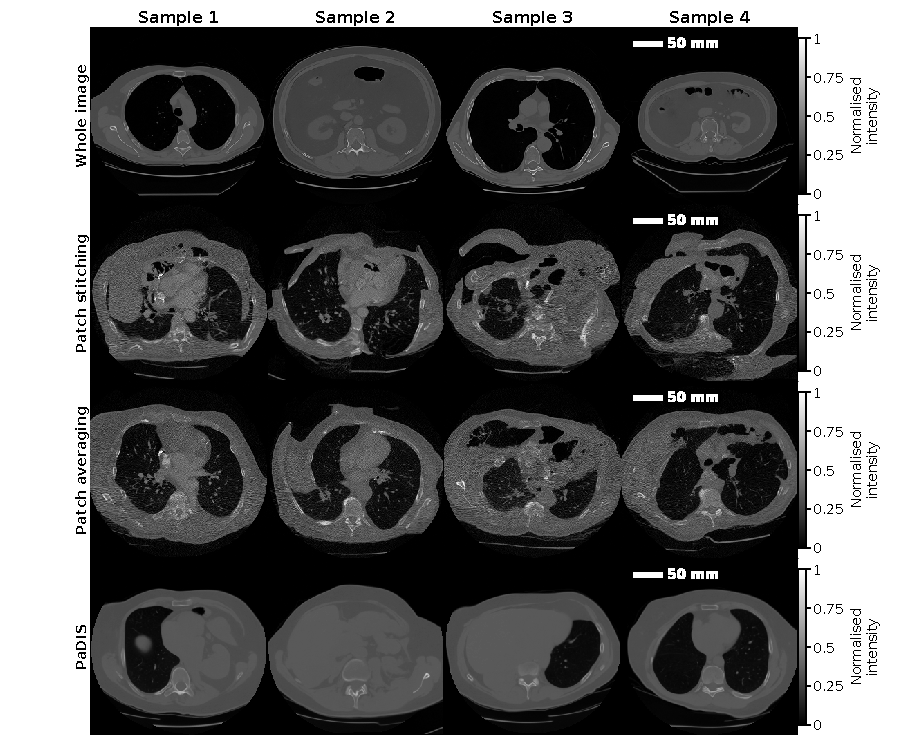
\includegraphics[width=\textwidth]{figure4_generation.pdf}
\caption{[Caption for Figure 4 generation results.]}
\label{fig:results-generation}
\end{figure}
\clearpage

\begin{figure}[p]
\centering
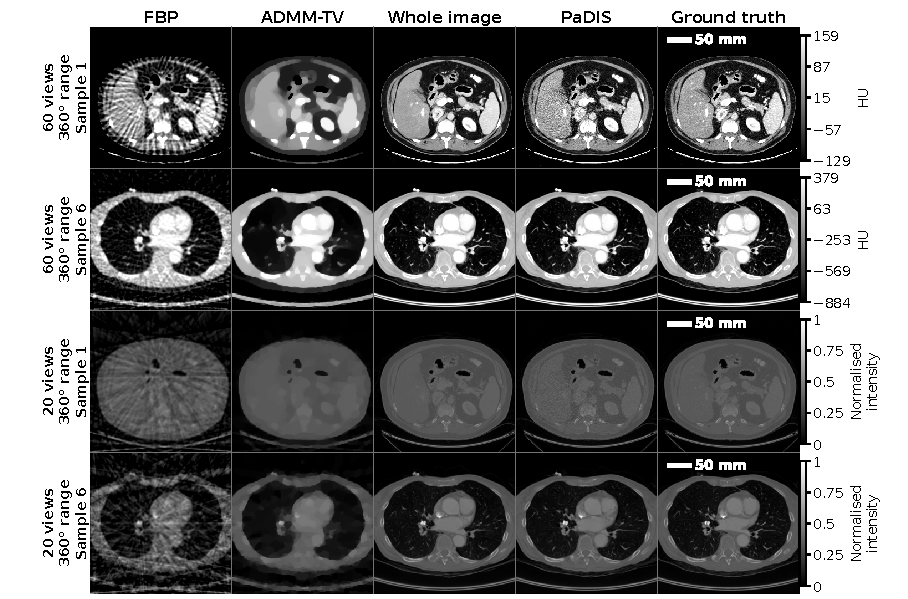
\includegraphics[width=\textwidth]{figure5_ct_reconstruction.pdf}
\caption{[Caption for Figure 5 CT reconstruction results.]}
\label{fig:results-ct-reconstruction}
\end{figure}
\clearpage

\begin{figure}[p]
\centering
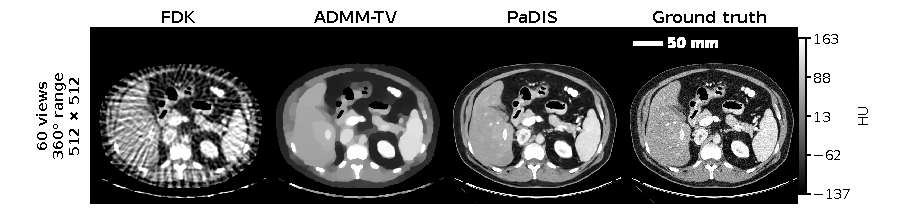
\includegraphics[width=\textwidth]{figure8_512_ct.pdf}
\caption{[Caption for Figure 8, 512 CT results.]}
\label{fig:results-512-ct}
\end{figure}
\clearpage

\begin{figure}[p]
\centering
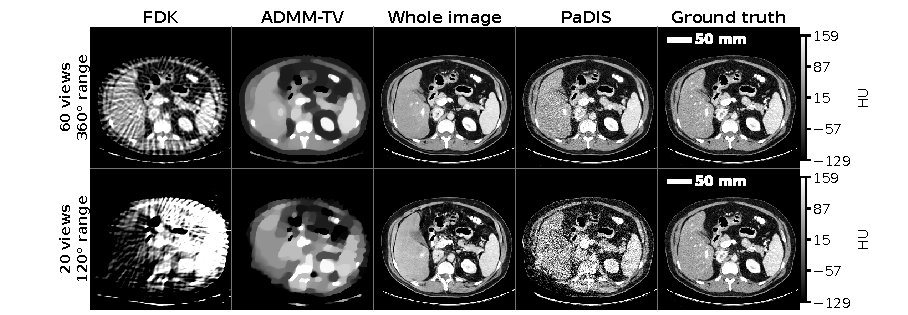
\includegraphics[width=\textwidth]{figureA10_extra_ct.pdf}
\caption{[Caption for Figure A10 additional CT results.]}
\label{fig:results-extra-ct}
\end{figure}
\clearpage

\begin{figure}[p]
\centering
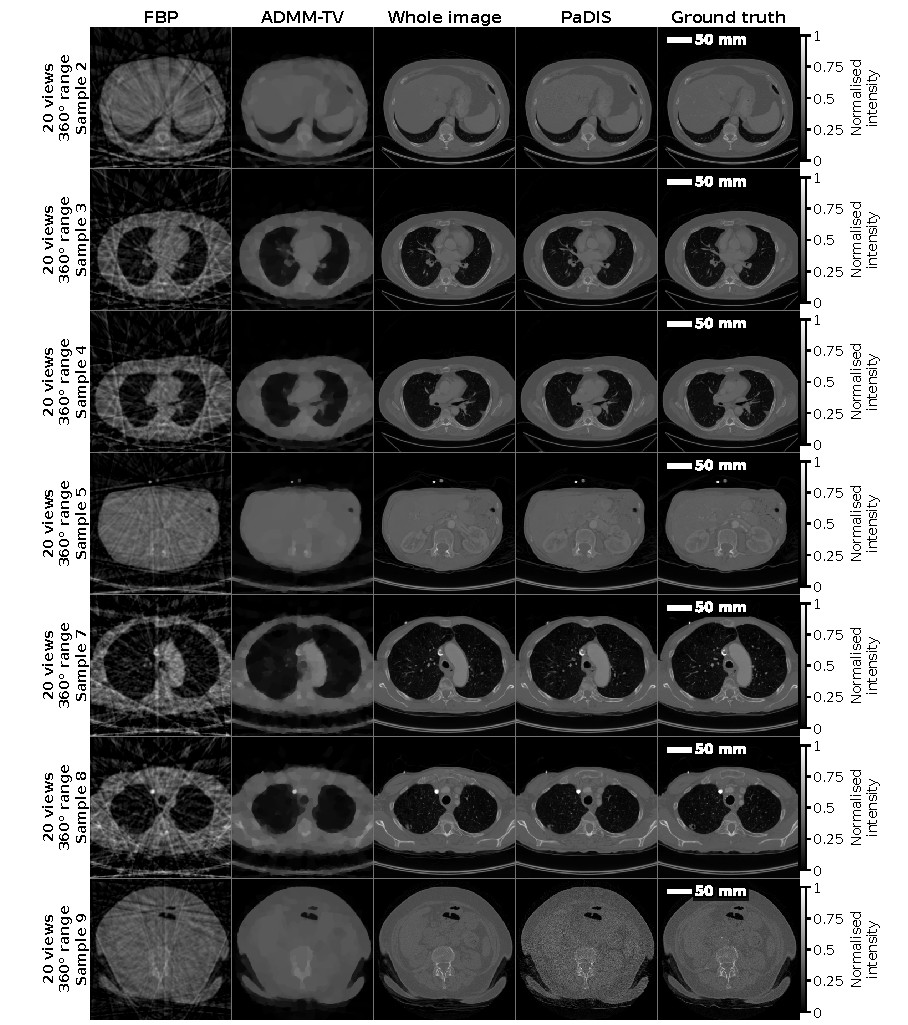
\includegraphics[width=\textwidth]{figureA1_ct20_additional.pdf}
\caption{[Caption for Figure A1, 20-view additional results.]}
\label{fig:results-ct20-additional}
\end{figure}
\clearpage

\begin{figure}[p]
\centering
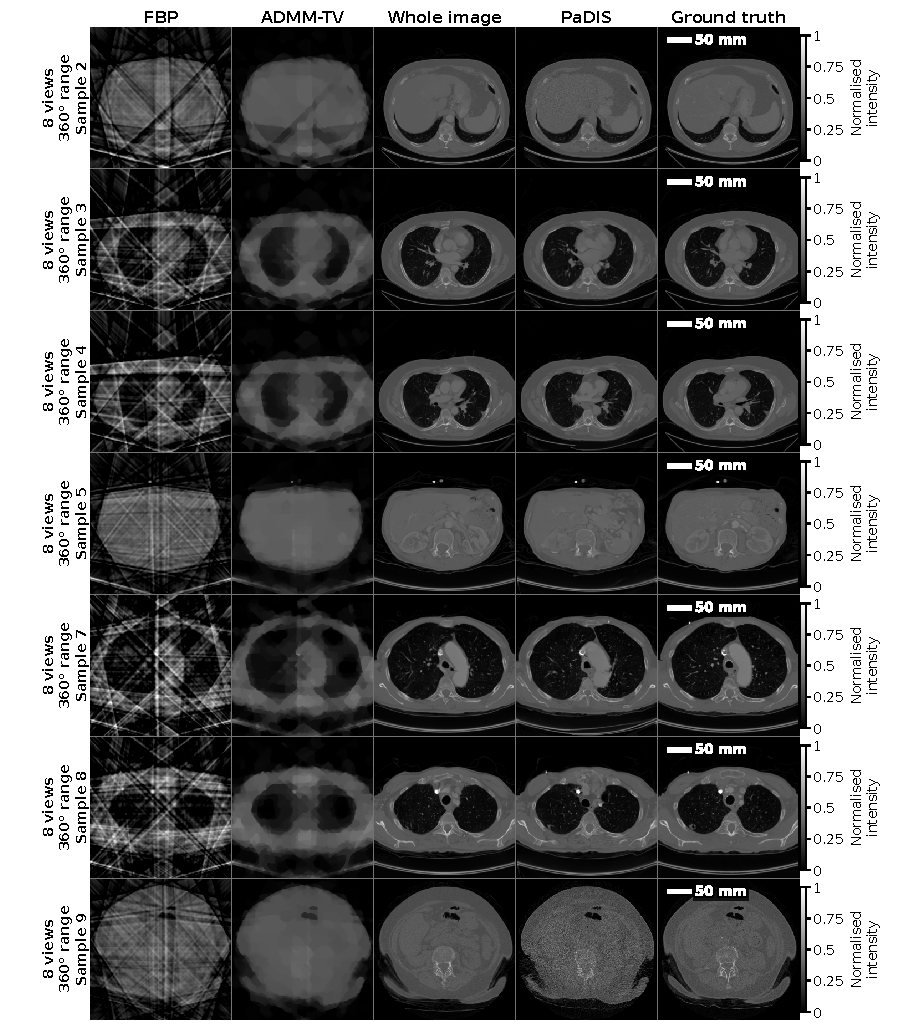
\includegraphics[width=\textwidth]{figureA2_ct8_additional.pdf}
\caption{[Caption for Figure A2, 8-view additional results.]}
\label{fig:results-ct8-additional}
\end{figure}
\clearpage

\begin{figure}[p]
\centering
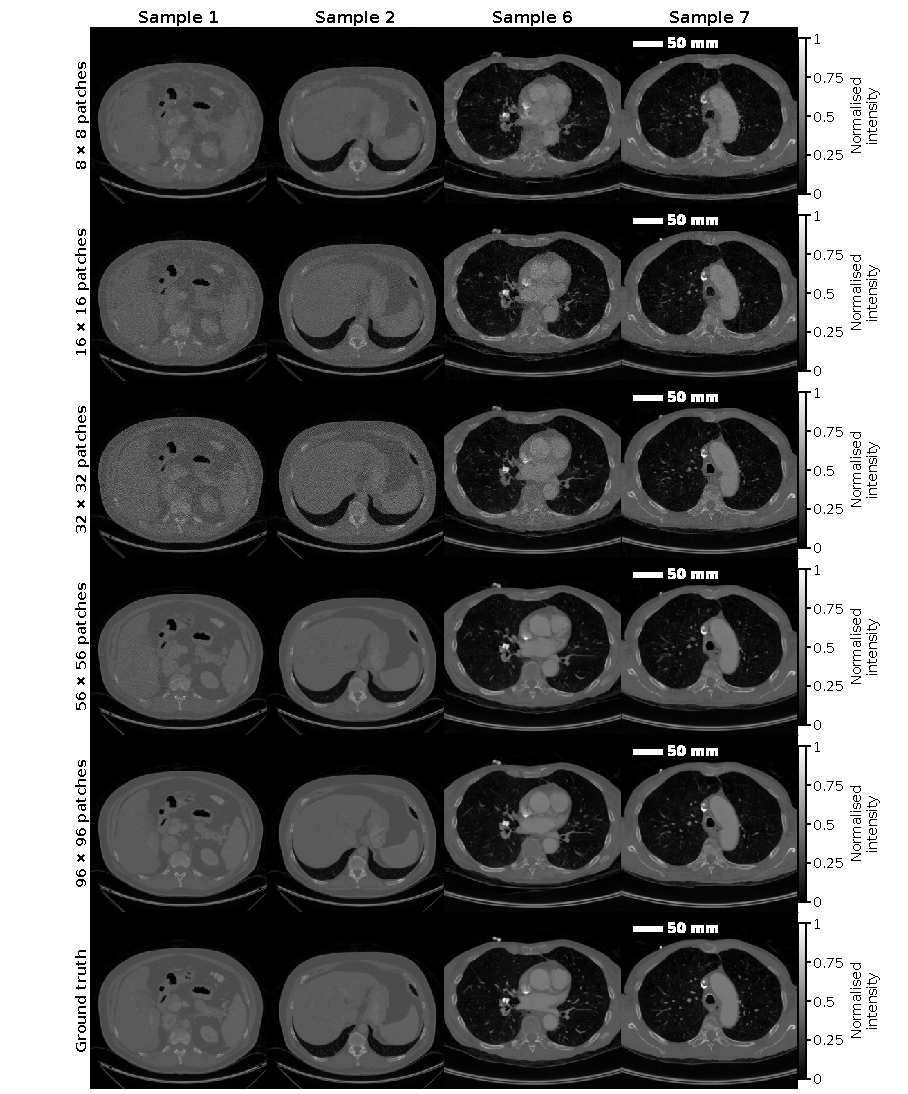
\includegraphics[width=\textwidth]{figureA5_patch_size.pdf}
\caption{[Caption for Figure A5 patch-size ablation.]}
\label{fig:results-patch-size}
\end{figure}
\clearpage

\begin{figure}[p]
\centering
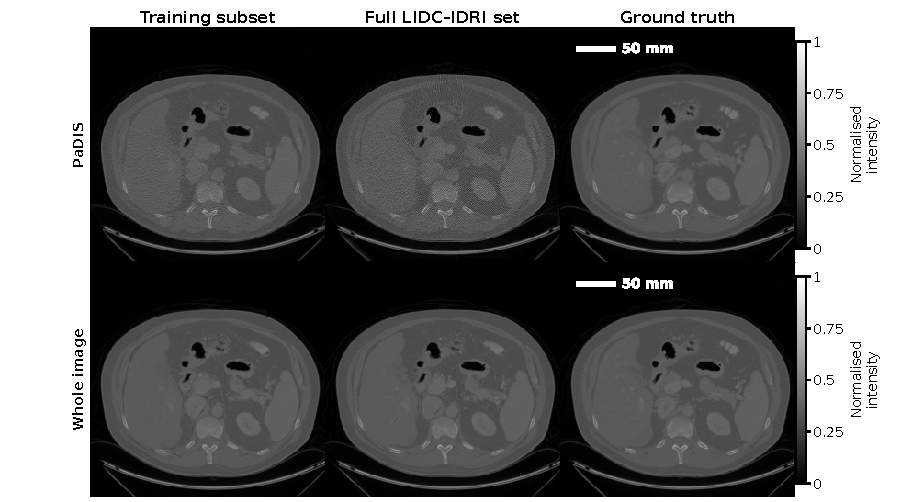
\includegraphics[width=\textwidth]{figureA6_dataset_size.pdf}
\caption{[Caption for Figure A6 dataset-size ablation.]}
\label{fig:results-dataset-size}
\end{figure}
\clearpage

\begin{figure}[p]
\centering
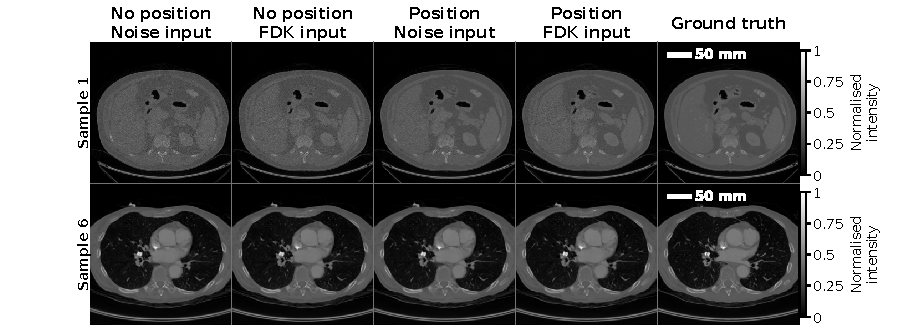
\includegraphics[width=\textwidth]{figureA7_position_encoding.pdf}
\caption{[Caption for Figure A7 position-encoding ablation.]}
\label{fig:results-position-encoding}
\end{figure}
\clearpage

\begin{figure}[p]
\centering
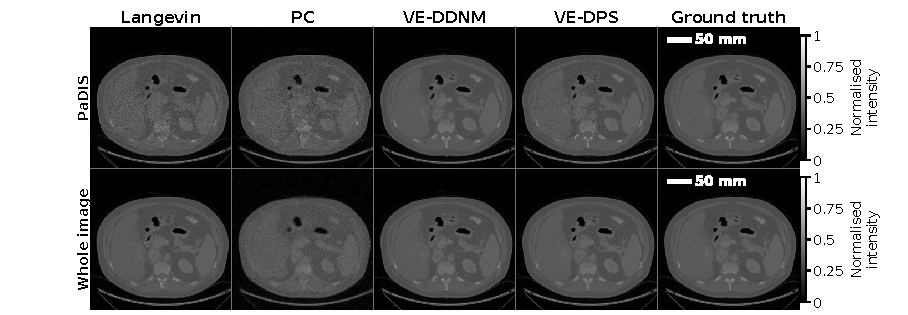
\includegraphics[width=\textwidth]{figureA8_sampling_methods.pdf}
\caption{[Caption for Figure A8 sampling-method comparison.]}
\label{fig:results-sampling-methods}
\end{figure}
\clearpage
